\section{System Design and Methodology}
\subsection{Research Design}

The main objective of this work is to develop a radar-based odometry system that estimates vehicle ego-motion using front-mounted mmWave radar sensors, combined with an IMU for rotation compensation.  
The motivation is to investigate radar as a cost-effective and robust alternative to vision- or LiDAR-based odometry, especially in conditions where these methods are prone to failure.  
This builds on prior evidence that radar can provide instantaneous ego-motion estimation through Doppler velocity cues \cite{EgoMotion_DopplerRadar}.  

The system processes radar point cloud data, enriched with range, angle, and Doppler velocity, to extract ego-velocity and reconstruct the vehicle’s trajectory.  
These outputs form a foundation for SLAM applications.  

As shown in Figure~\ref{fig:test_scenario}, two mmWave radar sensors were mounted at the front of the vehicle with overlapping fields of view to improve coverage and reduce ambiguity.  
This configuration served as the baseline validation scenario, chosen as a simple and controlled setup to verify the dual-radar concept before moving to more complex outdoor environments.  

\begin{figure}[!htbp]
    \centering
    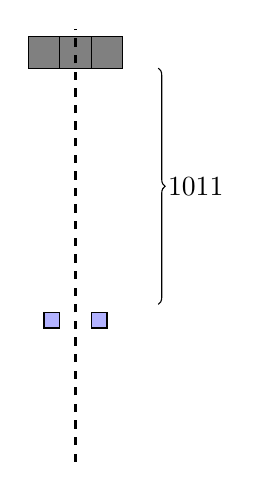
\begin{tikzpicture}
        \gokart{0}{0}{0}
    
        % Wall (three cubes)
        \draw[fill=gray] (-0.6,3) rectangle (-0.2,3.4);
        \draw[fill=gray] (-0.2,3) rectangle (0.2,3.4);
        \draw[fill=gray] (0.2,3) rectangle (0.6,3.4);
    
        % Dashed line from go-kart to wall (center axis)
        \draw[dashed, thick] (0,-2) -- (0,3.5);
    
        % Range brace annotation
        \draw [decorate, decoration = {brace, raise=10pt}] (0.7,3) -- (0.7, 0) node[pos=0.5,right=10pt,black]{\SIrange{10}{11}{\meter}};

        % Enlarged Radar sensor boxes
        \draw[fill=blue!30] (-0.4,-0.3) rectangle (-0.2,-0.1);
        \draw[fill=blue!30] (0.2,-0.3) rectangle (0.4,-0.1);
    \end{tikzpicture}
    \caption{Test scenario with dual front-mounted mmWave radar sensors.  
    This setup served as the baseline validation environment before moving to more complex scenarios.}
    \label{fig:test_scenario}
\end{figure}

The dual-radar arrangement increased point density and stability compared to single-radar approaches, aligning with multimodal strategies for robust state estimation \cite{Multimodal_Offroad,HighSpeed_Estimation}.  
By fusing Doppler-derived radial velocities with rotational information from the IMU, the system was designed to remain resilient in conditions where LiDAR- or camera-based odometry would degrade.  
Each radar stream was processed independently and then merged into a combined representation before entering the odometry pipeline.  

\subsubsection{Sub-Tasks}
The dual-radar objective implied several practical sub-tasks:  
\begin{itemize}
    \item Designing a modular pipeline to acquire and decode synchronized radar data from both sensors.  
    \item Investigating sensor configurations to balance field of view, chirp bandwidth, update rate, and detection density.  
    \item Developing mechanical mounts and selecting optimal sensor placement to ensure stability and maximize coverage.  
    \item Applying RANSAC filtering on Doppler velocities to reject dynamic points and outliers.  
    \item Implementing clustering methods to structure radar detections and isolate relevant features.  
    \item Leveraging additional sensor information (e.g., SNR, RCS, range validity) to optimize point cloud reliability.  
    \item Integrating Doppler velocity into the odometry estimation process.  
    \item Employing submap aggregation to mitigate sparsity and improve stability.  
    \item Performing ICP alignment between submaps aggregated from both sensors.  
    \item Evaluating the influence of the dual-sensor arrangement on odometry accuracy and robustness.  
    \item Validating the complete system on real-world driving scenarios.  
\end{itemize}

Taken together, these sub-tasks define the modular pipeline through which radar and IMU data are processed into ego-motion estimates.  
Each block in the pipeline corresponds to one or more of the identified tasks, from raw data acquisition and transformation, to filtering, clustering, and alignment.  
This modularity ensures that individual stages can be validated and tuned independently, while still contributing to the overall odometry framework.  
The complete processing chain is summarized in Figure~\ref{fig:dual_radar_pipeline}, which illustrates how the dual-radar inputs are merged with IMU measurements and progressively refined into robust ego-motion estimates.

\begin{figure*}[!htbp]
    \centering
    \resizebox{\textwidth}{!}{%
        \begin{tikzpicture}
            % Block style
            \tikzstyle{block} = [rectangle, draw, text width=4.5em, text centered, minimum width=6em, minimum height=4em]

            % Input branches
            \node[block] (radar1) {Radar\\Front Left};
            \node[block, below=1.2cm of radar1] (radar2) {Radar\\Front Right};

            % Physical transformation
            \node[block, right=of radar1] (transform1) {Rigid-Body\\Transform};
            \node[block, below=1.2cm of transform1] (transform2) {Rigid-Body\\Transform};

            % Merge
            \node[block, right=of transform1] (merge) {Radar Merge};

            % IMU (moved below radars)
            \node[block, below=1.2cm of transform2] (imu) {IMU};

            % Frame aggregator
            \node[block, right=of merge] (frame_aggr) {Frame\\Aggregator};
            \node[block, right=of frame_aggr] (coord_filter) {Filter\\$x,y,z$\\$\phi$, SNR};
            \node[block, right=of coord_filter] (ransac) {RANSAC};
            \node[block, right=of ransac] (doppler_filter) {Filter\\Dynamic Objects};
            \node[block, right=of doppler_filter] (clustering) {Clustering};
            \node[block, right=of clustering] (icp) {ICP};
            \node[block, right=of icp] (ego) {Ego-motion};

            % Self-speed estimator (below RANSAC)
            \node[block, below=1.5cm of ransac] (self_speed_estim) {Self-speed Estimator};
            \node[block, right=of self_speed_estim] (self_speed_kalman) {Kalman Filter};

            % Connections
            \draw[->] (radar1) -- (transform1);
            \draw[->] (radar2) -- (transform2);
            \draw[->] (transform1) -- (merge);
            \draw[->] (transform2) -| (merge);

            % Merge and IMU both feed into Frame Aggregator
            \draw[->] (merge) -- (frame_aggr);
            \draw[->] (imu) -| (frame_aggr);

            % Continue the pipeline
            \draw[->] (frame_aggr) -- (coord_filter);
            \draw[->] (coord_filter) -- (ransac);
            \draw[->] (ransac) -- (doppler_filter);
            \draw[->] (doppler_filter) -- (clustering);
            \draw[->] (clustering) -- (icp);
            \draw[->] (icp) -- (ego);

            % Self-speed estimator branch
            \draw[->] (ransac.south) -- (self_speed_estim.north);
            \draw[->] (self_speed_estim) -- (self_speed_kalman);

            % Bottom brace under radar2 (dual radar inputs only)
            \draw [decorate, decoration = {brace, mirror, raise=8pt}] 
                ([xshift=-2em,yshift=-1em]radar2.south west) -- 
                ([xshift=2em,yshift=-1em]radar2.south east)
                node[midway, below=12pt] {Dual-Radar Inputs};

            % Larger bottom brace under radars and IMU
            \draw [decorate, decoration = {brace, mirror, raise=16pt}] 
                ([xshift=-2em,yshift=-8.5em]radar2.south west) -- 
                ([xshift=2em,yshift=-1em]imu.south east)
                node[midway, below=20pt] {System Sensorial Inputs};
        \end{tikzpicture}
    }
    \caption{Dual-radar pipeline showing how radar and IMU inputs are merged into the frame aggregator before subsequent processing.}
    \label{fig:dual_radar_pipeline}
\end{figure*}

\newpage
The following sections detail the hardware setup, pipeline methodology, and experimental validation.
